
In this chapter, we aim to characterise transcript degradation and read truncation from long-read RNA-seq data. Transcript degradation from the 5' end results in truncated reads and a decrease in coverage with increasing distance from the 3' end for a given isoform. Thus, even though the observed degradation occurs from the 5' end, it is helpful to characterise degradation as the resultant decrease in coverage from the 3' end. We formalize the notion of degradation by defining the \textit{degradation rate}. 
\begin{definition}[Normalized coverage]
Let the maximum coverage over an isoform be $\mathrm{cov}_{\mathrm{max}}$ and the coverage at base $b$ be $\mathrm{cov}_b$. The normalized coverage of the isoform at base $b$ is defined as 
\begin{equation}
    \mathrm{ncov}_b=\frac{\mathrm{cov}_b}{\mathrm{cov}_{\mathrm{max}}}
\end{equation}
\end{definition}
\begin{definition}[Degradation rate]
Let $\mathrm{ncov}$ be the normalized coverage over an isoform, and $x$ be the distance in kb from the 3' end. The degradation rate of an isoform is defined as the rate of change in normalized coverage with respect to distance in kb from the 3' end of the isoform:
\begin{equation}
    d=\lim_{\Delta x\rightarrow 0} \frac{\Delta \mathrm{ncov}}{\Delta x}
\end{equation}
The degradation rate of an isoform at a base $b$ with distance $x_b$ away from the 3' end is the value of this limit evaluated at $x=x_b$. 
\end{definition}
To illustrate the concept of degradation rate, we visualise three different degradation rates for a hypothetical isoform of length 2 kb (Fig. \ref{fig:sec-2-hypo}).  
\begin{figure}[H]
    \centering
    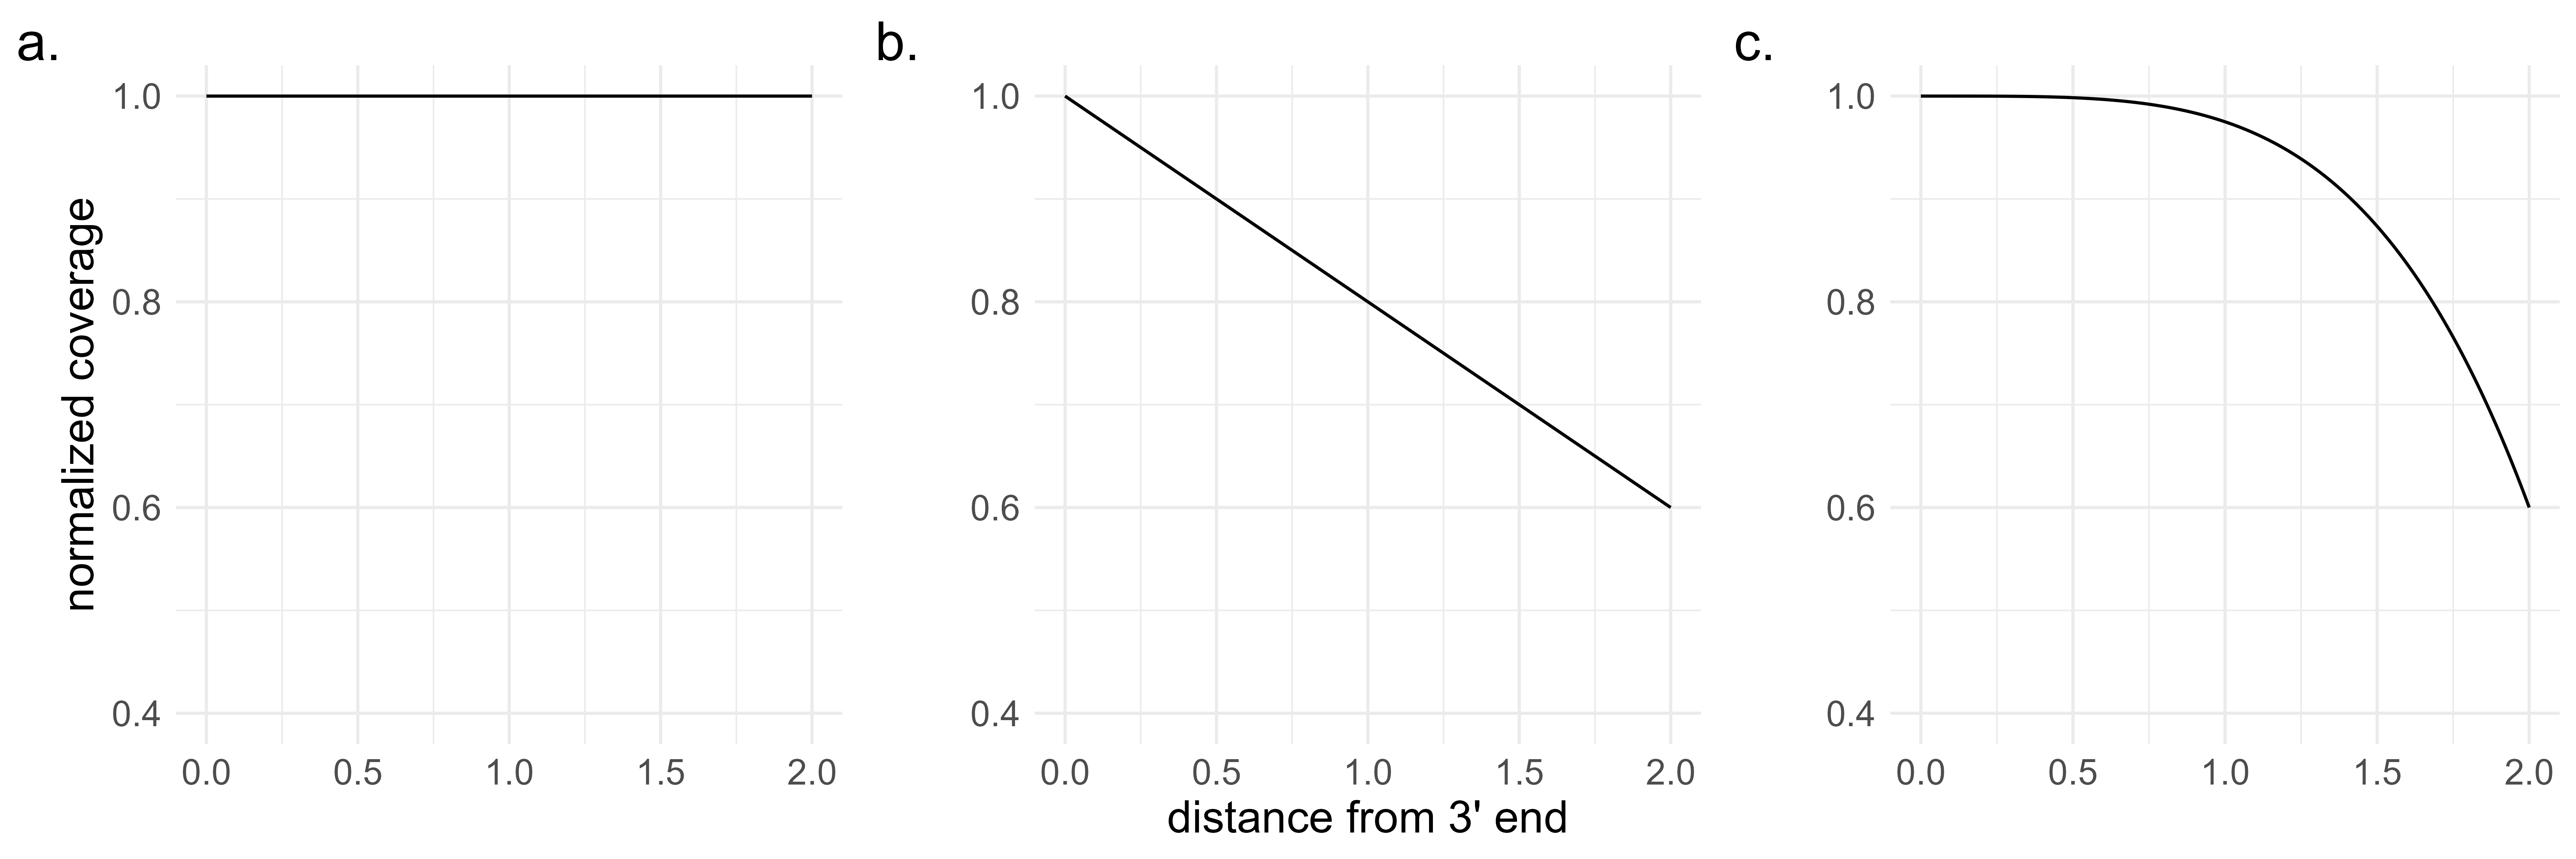
\includegraphics[width=\textwidth]{figures/sec-2-hypo.png}
    \caption[Degradation rates for a hypothetical isoform]{Degradation rates for a hypothetical isoform of length 2 kb.}
    \label{fig:sec-2-hypo}
\end{figure}
In the following sections, we describe our approach for estimating the degradation rate and present findings based on ONT long-read RNA-seq data from common cancer cell lines (A549, Hct116, HepG2, MCF7 and K562) as part of the SG-NEx project and a human embryonic stem cell line (H9). 

\section{Degradation rate estimation}

\subsection{Degradation by transcript features}

\subsection{Degradation in spike-ins}

\section{Coverage and read length distribution}


